% !TEX root = ../notes_missingsemester.tex
% Chapter 3: Dependencies & Project Structure
%%%%%%%%%%%%%%%%%%%%%%%%%%%%%%%%%%%%%%%%%%%%%%%%%%%%%%%%%%%%%%%%%%%%%%

% POST IMPROVEMENTS 2026:
% 1. Add a sequence diagram of pip's resolver to motivate lock files visually.
% 2. Provide a pre-baked v0.2 reference repo so catch-up takes a single clone. (maybe solved with tags already)
% 3. % TODO: Good add-on teaching on how they release their own first package of something. 



\index{dependencies}\index{virtualenv}\index{pip}\index{project structure}\index{12-factor app}
\chapter{Dependencies \& Structure}
\printchapterversion{03_dependencies_structure}
\newthought{Works on my machine.}

% ==============================================================================================
% BLOCK 1: INTRODUCTION
% ==============================================================================================

\section{The Why}\index{reproducibility}\index{requirements.txt}\index{setup-server.sh}\index{.env}

Block~2 left us with a PixelWise repository on GitHub and a server that has
Git and Python installed.
Both machines share the same history, both can pull from \texttt{origin},
and the workflow that moves code between them is in place.
What is still missing is the layer beneath the code: the system packages, the language runtime, the libraries, and the secrets
your application reads (installed or provisioned by \texttt{setup-server.sh} and recorded in \texttt{.env}/\texttt{.env.example}).

\marginnote{\newthought{PixelWise} now lives on GitHub and on both machines,
but the repository contains only \texttt{README.md} and \texttt{.gitignore}.
Before we can write application code, we need a reproducible way to install
everything the project depends on, so that \texttt{dev} and \texttt{prod}
stay in sync without human memory.
Use \texttt{setup-server.sh} to provision system packages and the runtime, and
keep secrets and runtime configuration in \texttt{.env.example} (copied to \texttt{.env}).}

\newthought{Kaltstart Capabilities}\index{PixelWise},
Your colleague clones the repository, runs the code, and immediately hits an
\texttt{Error}.
You installed a package with a specific version months ago and forgot.
They did not.
The remainder of the day is spent debugging an artefact of the install
history rather than contributing real value to the program itself.
At the end of this third block we want any fresh VM to go from empty
to ready to code with a small, fixed sequence of commands.
The two halves of that sequence are the load-bearing idea of the chapter:
system packages on one side, Python packages on the other,
version controlled in different files. 


\vspace{1.5em}
\begin{figure}
\centering
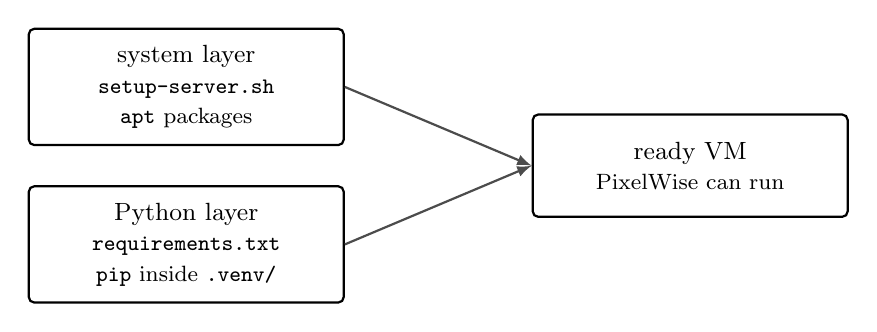
\begin{tikzpicture}[
    every node/.style={font=\small, align=center},
    box/.style={rectangle, draw=black, thick, rounded corners=2pt, minimum width=4.0cm, minimum height=1.3cm, inner sep=6pt},
    arr/.style={-latex, thick, black!70}
]
\node[box] (sys) at (0, 1.0) {system layer\\\footnotesize \texttt{setup-server.sh}\\\footnotesize \texttt{apt} packages};
\node[box] (py)  at (0, -1.0) {Python layer\\\footnotesize \texttt{requirements.txt}\\\footnotesize \texttt{pip} inside \texttt{.venv/}};
\node[box] (env) at (6.4, 0) {ready VM\\\footnotesize PixelWise can run};
\draw[arr] (sys.east) -- (env.west);
\draw[arr] (py.east)  -- (env.west);
\end{tikzpicture}
\caption{Two layers, two files. \protect\texttt{setup-server.sh} provisions the operating system; \protect\texttt{requirements.txt} 
provisions Python inside an isolated virtual environment. Together they reconstruct the environment from scratch on any fresh VM. 
System packages, the things you install with \protect\texttt{apt}\protect\index{apt},
are captured in a shell script called \protect\texttt{setup-server.sh}\protect\index{setup-server.sh}.
Python packages, the libraries your application imports,
are captured in \protect\texttt{requirements.txt}\protect\index{requirements.txt} and installed
inside an isolated virtual environment.
The two files are committed to Git, run on either machine,
and produce identical environments without any further intervention.}
\label{fig:two_layers}
\end{figure}



\newpage
\subsection{Hands On Experience}

\newthought{Consider this scenario:} you hand your PixelWise repository to a
classmate at the end of the day.
They clone it, type \texttt{python3 train.py} without running the provisioning script \texttt{setup-server.sh},
and immediately hit \texttt{ModuleNotFoundError: No module named 'sklearn'}.
You tell them to install scikit-learn.
They do, but they get version 2.0 while you wrote the code against 1.4.
The training script crashes with a different error.
By the time the original problem is fixed,
a few hours are gone and neither of you has touched the actual code nor added any value.

\marginnote{\newthought{The two-command promise.}
A well-managed project lets any new developer go from clone to running code
with two commands: create the virtual environment and install from a pinned
requirements file.
No guessing, no mails or messages asking ``which version of numpy do I need?''
This block is what makes that promise hold.}

\newthought{Reproducible projects} do not require remembering, asking, or guessing.
The exact set of packages, the exact versions, the exact configuration
contract, are written down once, committed to Git, and replayed on any
machine that has the script and the file.

\marginnote{\newthought{Outside the classroom,} the same files are how cloud
deployment works in practice.
A continuous-integration runner clones the repository, executes the setup
script (for example, \texttt{setup-server.sh}), installs from \texttt{requirements.txt}, 
and runs the tests.
The reproducibility you build for two VMs scales without modification
to a hosted server, a colleague's laptop, or a CI runner you have never seen.}

\newthought{This third block} introduces dependency management and project
structure for PixelWise.
By the end you will have
\begin{itemize}
    \item captured system-level setup in a reproducible shell script,
    \item created and activated a Python virtual environment,
    \item installed packages with \texttt{pip} and pinned them in \texttt{requirements.txt},
    \item separated secrets from code using \texttt{.env} and \texttt{.env.example},
    \item scaffolded the PixelWise project directory,
    \item and audited your dependencies for known security vulnerabilities.
\end{itemize}




% ==============================================================================================
% BLOCK 2: CONCEPTS AND PRACTICE
% ==============================================================================================






\newpage
\section{Optional Exercise: Catch Up to \texttt{v0.1}}\index{exercises}\index{Git!tag}\index{recovery}

\newthought{Catching up via the reference tag.}\index{Git!tag}\index{recovery}
From this block onwards, the GitHub repository is the safety net.
The course maintains a public reference repository at
\url{https://github.com/schutera/pixelwise} with a tag at the end of every block.
\texttt{v0.1} marks the end of Block~2; \texttt{v0.2} will mark the end of
this block.
If you joined late, missed Block~2, or your repository has drifted from a
known good state, reset to the previous tag rather than redoing every prior
exercise.

\marginnote{\newthought{Tag map.}\index{Git!tag}
\texttt{v0.1} is the end of Block~2,
\texttt{v0.2} is the end of this block,
\texttt{v0.3} the end of Block~4, and so on.
Every tag is a complete, runnable state of PixelWise.
Browse them at
\url{https://github.com/schutera/pixelwise/tags}.}

\newthought{The model:} pull from \texttt{schutera/pixelwise}, push to your
own \texttt{<you>/pixelwise}. The reference repository is read-only for
you; the place you commit to is your personal copy on GitHub. The steps
below assume nothing from Block~2 is in place, so the exercise is fully
self-contained.

\newthought{Create an empty \texttt{pixelwise} repository on GitHub} under
your own account. Log in to GitHub, click New repository, name it
\texttt{pixelwise}, and leave it empty, no README, no \texttt{.gitignore},
no licence, since the push step below will populate it. Without this
repository the \texttt{git remote set-url} URL points at a path GitHub
cannot find, and the first push reports \texttt{does not appear to be a
git repository}.

\newthought{Restore \texttt{B1-complete} on \texttt{dev}} so you start from
the same baseline as everyone else, with Ubuntu installed and the user
account in place but nothing on top.

\newthought{Install Git, configure your identity, and generate a separate
SSH key for GitHub} on the fresh VM. \texttt{B1-complete} predates Block~2,
so the new VM has no \texttt{git} binary and no Git config. It does already
have \texttt{\textasciitilde/.ssh/id\_ed25519} and
\texttt{\textasciitilde/.ssh/id\_ed25519.pub} from Block~1, the key pair
you use to log in to \texttt{prod}. The \texttt{-f} flag below writes the
new key to a distinct path, so the existing prod-login key files stay
byte-for-byte intact on disk and your password-less SSH into \texttt{prod}
keeps working:

\begin{verbatim}
sudo apt update && sudo apt install -y git
git config --global user.name  "Your Name"
git config --global user.email "your@email.com"
ssh-keygen -t ed25519 -C "your@email.com" \
    -f ~/.ssh/id_ed25519_github
ls -l ~/.ssh/id_ed25519*
cat ~/.ssh/id_ed25519_github.pub
\end{verbatim}

\marginnote{\newthought{Sanity check.}\index{SSH!key}
\texttt{ls -l} should now list four files under
\texttt{\textasciitilde/.ssh/}: the \texttt{id\_ed25519} pair from Block~1
and the \texttt{id\_ed25519\_github} pair you just generated. If the
Block~1 files are missing, you accepted the default path during
\texttt{ssh-keygen} and overwrote the prod key. Restore
\texttt{B1-complete} and rerun the step with the \texttt{-f} flag.}

\marginnote{\newthought{Add the key to GitHub.}\index{SSH!key}
Copy the entire \texttt{ssh-ed25519 \ldots} line printed by
\texttt{cat \textasciitilde/.ssh/id\_ed25519\_github.pub}, go to Settings,
then SSH and GPG keys, then New SSH key on GitHub, give it a title like
\texttt{pixelwise-dev-vm}, and paste.}

\newthought{Tell SSH which key to use for github.com.}\index{SSH!config}
With two keys in \texttt{\textasciitilde/.ssh/}, SSH may offer the
prod-login key first and GitHub authenticates you as the wrong account, or
fails outright. Worse, if \texttt{ssh-agent} has already cached the
prod-login key, it gets offered before any \texttt{IdentityFile} on disk,
and the symptom is a misleading
\texttt{git@github.com:<you>/pixelwise.git does not appear to be a git
repository}. Open (or create) \texttt{\textasciitilde/.ssh/config} in
\texttt{nano} and add an entry that pins the GitHub key to github.com and
bypasses the agent for that host:

\begin{verbatim}
nano ~/.ssh/config
\end{verbatim}

Paste the following block at the end of the file, then save and exit nano with
\texttt{Ctrl+X, Y, Enter}:

\begin{verbatim}
Host github.com
    HostName github.com
    User git
    IdentityFile ~/.ssh/id_ed25519_github
    IdentitiesOnly yes
    IdentityAgent none
\end{verbatim}

\newthought{Lock down the file permissions.}\index{SSH!config}
SSH refuses to read \texttt{config} if it is world- or group-readable, so
tighten it to the owner only:

\begin{verbatim}
chmod 600 ~/.ssh/config
\end{verbatim}

\marginnote{\newthought{Why \texttt{IdentityAgent none}?}\index{ssh-agent}
\texttt{IdentitiesOnly yes} alone tells \texttt{ssh} to ignore extra agent
keys, but in practice some agent setups still offer them first.
\texttt{IdentityAgent none} is the belt-and-braces fix: for connections to
github.com, skip the agent entirely and read the key from the file you
named, period. Other hosts, including \texttt{prod}, are unaffected and
still use the agent normally, so password-less SSH into \texttt{prod} keeps
working.}

\marginnote{\newthought{Already polluted the agent?}\index{ssh-agent}
If you ran \texttt{ssh-add} earlier in the session and \texttt{ssh-add -l}
now lists more than one key, drop them all from the agent and reload only
the GitHub key:
\\[0.5em]
\texttt{ssh-add -D}\\
\texttt{ssh-add \textasciitilde/.ssh/id\_ed25519\_github}
\\[0.5em]
\texttt{ssh-add -D} only forgets the keys held in agent memory; the files
in \texttt{\textasciitilde/.ssh/} are not touched. Re-add the prod key
later with \texttt{ssh-add \textasciitilde/.ssh/id\_ed25519} when you next
log in to \texttt{prod} if you prefer not to retype the passphrase.}

\newthought{Run the verification handshake.}\index{SSH!known\_hosts}
The first SSH connection to
GitHub asks you to confirm GitHub's host fingerprint and writes it into
\texttt{\textasciitilde/.ssh/known\_hosts}:

\begin{verbatim}
ssh -T git@github.com
\end{verbatim}

Type \texttt{yes} when prompted to trust the fingerprint. GitHub then
answers \texttt{Hi <you>! You've successfully authenticated, but GitHub
does not provide shell access.} The shell-access line sounds like an
error but is the intended response: GitHub allows Git operations over
SSH, not interactive shells.

\newthought{Catch-up procedure on \texttt{dev}.}
With the empty repository in place and the key registered, clone the
reference repository, rewind \texttt{main} to the \texttt{v0.1} tag, point
\texttt{origin} at your own empty repository, and push:

\begin{verbatim}
cd ~
git clone https://github.com/schutera/pixelwise.git
cd pixelwise
git reset --hard v0.1
git remote set-url origin \
    git@github.com:<you>/pixelwise.git
git push -u origin main
git push --tags
\end{verbatim}

\marginnote{\newthought{Why \texttt{reset -{}-hard}?}\index{Git!reset}
The clone lands you on the reference repository's current \texttt{main},
which is ahead of \texttt{v0.1}. \texttt{git reset -{}-hard v0.1} moves
your local \texttt{main} back to the tagged commit, discarding the later
ones, so the working tree matches the end-of-Block~2 state exactly. There
is no work to lose because you have not committed anything yet.}

\newthought{Mirror it on \texttt{prod}.}
By the end of Block~2, PixelWise also lived on the production VM at
\texttt{/opt/pixelwise}. Restore \texttt{B1-complete} on \texttt{prod} as
well, install \texttt{git}, then clone the reference repository to its
permanent home and rewind \texttt{main} to \texttt{v0.1}:

\begin{verbatim}
sudo apt update && sudo apt install -y git
sudo mkdir -p /opt/pixelwise
sudo chown produser:produser /opt/pixelwise
git clone https://github.com/schutera/pixelwise.git \
    /opt/pixelwise
cd /opt/pixelwise
git reset --hard v0.1
\end{verbatim}

\marginnote{\newthought{No SSH key on \texttt{prod}.}\index{SSH!key}\index{Git!HTTPS clone}
\texttt{prod} only ever pulls; it never pushes, so an HTTPS clone of a
public repository is enough and no SSH key needs to be registered with
GitHub. Skip the \texttt{ssh-keygen} ceremony you just did on \texttt{dev}.
If your repository is private, or you later need to push from \texttt{prod},
generate a separate key on \texttt{prod} and add it to GitHub the same way.}

\marginnote{\newthought{Already have a fork?}\index{Git!fork}
If your own fork already carries the \texttt{v0.1} tag, swap the URL for
\texttt{git@github.com:<you>/pixelwise.git} on \texttt{dev} and the HTTPS
equivalent on \texttt{prod}, so push and pull continue to target your account
rather than the reference repo.}

You are now at the state where Block~2 ended, with both VMs aligned, ready
to start Block~3.


\newpage
\section{The Setup Script}\index{setup-server.sh}\index{provisioning}

\newthought{Provisioning a server} is the act of turning a freshly installed
operating system into one that can run your application.
So far it has been done by typing \texttt{sudo apt install} commands at the
prompt and reading their output.
That works for one-time setups, it does not scale.
Software is meant to be scaled.

\marginnote{\newthought{Configuration management} is a whole discipline that
grew from this small itch.
Ansible\index{Ansible}, Salt, and Puppet declare the desired state of a
machine in a structured format and reconcile the live system to match.
\texttt{setup-server.sh} is the entry-level version: a script you can read
end to end. The principle is the same.\\
Ansible: \url{https://docs.ansible.com/}}

\newthought{The setup script} is a plain Bash\index{Bash} file that captures every
\texttt{apt install} the project needs.
It lives in the repository alongside the code and is run on any fresh VM
to bring it up to speed:

\begin{verbatim}
#!/bin/bash
# setup-server.sh: provision a fresh server VM
set -euo pipefail

sudo apt update
sudo apt install -y git python3 python3-pip \
    python3-venv curl
\end{verbatim}

\marginnote{\newthought{The shebang line}\index{shebang} \texttt{\#!/bin/bash}
tells the kernel which interpreter to use when you run the file directly.
Without it, the file is read as a sequence of commands by whichever shell
happens to invoke it, which on Ubuntu is usually \texttt{dash}, not Bash,
and the two differ in subtle ways that surface only when something breaks.}

\newthought{The first line of the body,} \texttt{set -euo pipefail}\index{set -euo pipefail},
makes the script fail loudly.
\texttt{-e} aborts on the first error, \texttt{-u} aborts on an undefined variable,
and \texttt{-o pipefail} propagates a failed command in the middle of a pipeline
rather than letting a successful command later on mask it.
Half-configured machines are a common cause of mysterious bugs;
the four-character preamble eliminates most of them.

\marginnote{\newthought{Idempotence}\index{idempotence} is the property that
running a script twice yields the same result as running it once.
\texttt{apt install} is idempotent by default: an already-installed package
is a no-op. So re-running is always safe, and the script can be used to fix a machine that has drifted.}

\newthought{Mark it executable} and run it:

\begin{verbatim}
chmod +x setup-server.sh
./setup-server.sh
\end{verbatim}

\newthought{See how version control already pays off.}
The script is committed to Git, so when the VM is rebuilt or a new team
member joins, \texttt{bash setup-server.sh} reproduces the exact same
environment.
The commands you typed once are written down where the next person can find them.


\newpage
\section{Exercise: The Setup Script}\index{exercises}

\newthought{With the setup script motivated above,} put it on the \texttt{dev} VM.
At the root of the PixelWise repository, that is \texttt{\textasciitilde/pixelwise/}
where you ran \texttt{git init} in Block~2, create a file called
\texttt{setup-server.sh} that captures the system packages installed manually
in Block~2:

\marginnote{\newthought{Why at the repo root?}\index{repository layout}
Provisioning is a project-wide concern, not the responsibility of any single
subdirectory, so \texttt{setup-server.sh} sits next to \texttt{README.md} and
\texttt{.gitignore} where anyone cloning the repository will spot it
immediately. Open the file with \texttt{nano \textasciitilde/pixelwise/setup-server.sh}
or your editor of choice and paste the contents below.}

\begin{verbatim}
#!/bin/bash
set -euo pipefail

sudo apt update
sudo apt install -y git python3 python3-pip \
    python3-venv curl
\end{verbatim}

\marginnote{\newthought{(Optional) Try it on a fresh VM.}\index{provisioning}
The real test of the script is on a machine that has not seen the commands
yet.
A second \texttt{prod} VM, restored from the \texttt{B1-complete} image,
clones the repository, runs \texttt{bash setup-server.sh}, and provisions
end to end without you typing a single \texttt{apt install}.}

\newthought{Mark it executable and run it.}
On a machine that already has the packages, every \texttt{apt install} is a
no-op; the script reports nothing to do, which is the desired outcome of
an idempotent provisioning step:

\begin{verbatim}
chmod +x setup-server.sh
./setup-server.sh
\end{verbatim}

\newthought{Commit it.} This is the first file that makes provisioning reproducible:

\begin{verbatim}
git add setup-server.sh
git commit -m "Add server provisioning script"
git push
\end{verbatim}



% ==============================================================================================
\newpage
\section{Virtual Environments}\index{virtualenv}\index{venv}

\newthought{A virtual environment} is an isolated Python installation.
Each project gets its own set of packages, independent of every other project
and of the system Python.
The mechanism is local: a directory, by convention called \texttt{.venv/},
that holds an interpreter, a copy of \texttt{pip}, and every library the
project depends on.
Activating the environment rewrites your shell's \texttt{PATH} so that
\texttt{python} and \texttt{pip} resolve to the local copies.

\begin{verbatim}
python3 -m venv .venv
source .venv/bin/activate
\end{verbatim}

\marginnote{\newthought{Why isolation?}\index{isolation}
Project A needs \texttt{numpy==1.24}; project B needs \texttt{numpy==2.0}.
Without per-project environments, one of them breaks the moment the other
is installed.
With virtual environments, both coexist on the same machine and make it easy for you to switch between projects seamlessly.}

\newthought{The directory is large} and machine specific, often 50 to 200\,MB.
Thus it is listed in \texttt{.gitignore}: never commit it.
A teammate clones the repository, creates their own \texttt{.venv}, installs
from \texttt{requirements.txt}, and ends up with the same packages without
ever copying the binary contents.

\newthought{Verify the switch.}
After activation, \texttt{which python} should report a path inside
\texttt{.venv/bin/}, and \texttt{pip list} should show only \texttt{pip}
and \texttt{setuptools}:

\begin{verbatim}
which python
# /home/user/pixelwise/.venv/bin/python

pip list
# Package    Version
# ---------- -------
# pip        24.0
# setuptools 69.5.1
\end{verbatim}

A fresh environment starts empty.
Every package you install from this point is tracked and intentional.
\texttt{deactivate} returns the shell to the system Python.

\marginnote{\newthought{The data science ecosystem} often uses
\texttt{conda}\index{conda} instead of \texttt{venv}.
Conda manages both Python packages and system-level libraries like CUDA or
MKL, which makes it popular for GPU workflows.
For web projects, \texttt{venv} is the lighter and more standard choice.\\
Conda: \url{https://docs.conda.io/}}

\newthought{The rule is simple:} every project gets its own \texttt{.venv}.
Activate it before you work; deactivate when you are done.
The one-time cost is a directory and a command;
the ongoing benefit is never debugging a version conflict between two
unrelated projects on the same laptop.



% ==============================================================================================
\newpage
\section{Exercise: The Virtual Environment}\index{exercises}

\newthought{With the rationale for isolation in mind,} create one on the
\texttt{dev} VM, inside the PixelWise repository:

\begin{verbatim}
cd ~/pixelwise
python3 -m venv .venv
source .venv/bin/activate
\end{verbatim}

\marginnote{\newthought{Notice the prompt change.}\index{shell prompt}
After activation, your shell prompt usually gains a \texttt{(.venv)} prefix
to remind you which environment is active.
If you ever wonder whether you are inside the project's environment,
the prompt is the first place to look; \texttt{which python} is the second.}

\newthought{Verify the switch.}
\texttt{which python} should print a path inside \texttt{.venv/bin/}.
\texttt{pip list} should show only \texttt{pip} and \texttt{setuptools}:

\begin{verbatim}
which python
pip list
\end{verbatim}

A fresh environment is empty by design.
The next exercise fills it with intent.

\newthought{Add the environment to \texttt{.gitignore}.}
The \texttt{.venv/} directory must never be committed.
Open the \texttt{.gitignore} from Block~2 and confirm \texttt{.venv/} is
listed; if not, add it now. You will notice that currently we 
ignore \texttt{*.py} python files, but in future you do not want to ignore those, so remove that line:

\begin{verbatim}
.venv/
\end{verbatim}

\marginnote{\newthought{Read the diff.}\index{Git!diff}
\texttt{git diff .gitignore} shows what you added compared to the Block~2
version.
Reading the diff before committing is the habit that catches accidental
changes early; running it once now is muscle memory you will reuse every
day for the rest of the course.}

Run \texttt{git status}. The only change shown should be the
\texttt{.gitignore} edit itself, even though \texttt{.venv/} sits right
next to it on disk with hundreds of files inside. That silence is
\texttt{.gitignore} doing its job: the absence of \texttt{.venv/} in the
output is the demonstration, not a missing piece.

\newthought{Commit the change.}
With the diff read and \texttt{git status} clean of surprises, record the
update so the next exercise starts from a known state:

\begin{verbatim}
git add .gitignore
git commit -m "Ignore .venv/ and stop ignoring *.py"
git push
\end{verbatim}



% ==============================================================================================
\newpage
\section{Managing Packages with pip}\index{pip}\index{requirements.txt}
% TODO: Good add-on teaching on how they release their own first package of something. 


\newthought{pip is the package installer} for Python.\index{PyPI}
It downloads packages from PyPI, the Python Package Index at
\url{https://pypi.org/}, and installs them into the active environment.
The core cycle has three commands:

\begin{verbatim}
pip install scikit-learn joblib python-dotenv
pip freeze > requirements.txt
pip install -r requirements.txt
\end{verbatim}

\marginnote{\newthought{The three packages.}\index{scikit-learn}\index{joblib}\index{python-dotenv}
\texttt{scikit-learn} provides the classifier PixelWise will train and
serve.
\texttt{joblib} saves and loads trained models to disk as \texttt{.pkl}
files.
\texttt{python-dotenv} reads \texttt{.env} files into environment
variables so secrets stay out of code.}

\marginnote{\newthought{Read these three lines as a contract.}
The first installs into the environment.
The second writes a snapshot of it to a text file.
The third reconstructs the same environment from the file on any machine.
Together they are the reproducibility layer for your programming environment.}

\newthought{\texttt{pip install}} downloads each named package and its
dependencies and places them in \texttt{.venv/}.
\texttt{pip freeze} prints every installed package with its exact version,
including transitive dependencies you never asked for directly.
\texttt{pip install -r} reads such a file and installs everything in it,
the step that turns a captured environment back into a live one.

\subsection{Anatomy of \texttt{requirements.txt}}

\newthought{One package per line,} pinned to an exact version:

\begin{verbatim}
scikit-learn==1.4.0
joblib==1.3.2
python-dotenv==1.0.1
\end{verbatim}

\marginnote{\newthought{Version specifiers}\index{semantic versioning}.
\texttt{==} pins exactly, \texttt{>=} sets a floor, \texttt{\~{}=} allows
patch updates: \texttt{\~{}=1.4.0} means \texttt{>=1.4.0, <1.5.0}.
For maximum reproducibility, pin everything with \texttt{==}.
Looser specifiers are appropriate for libraries that other projects depend on,
which is not where most of your work lives.\\
Semantic versioning: \url{https://semver.org}}

\newthought{Pinning matters} because packages are a moving target.
A package you install today as \texttt{numpy>=1.24} may resolve to
\texttt{1.27} tomorrow, with new features added, new behaviour, new bugs, and possibly new
security advisories. Packages are software, and they are subject to change; just the same as your own project.
Pinning to \texttt{==1.24.3} freezes the resolution and makes switching to newer versions a deliberate act.

\marginnote{\newthought{Security auditing.}\index{pip audit}\index{CVE}
Your dependencies have their own dependencies, and any of them can harbour
known vulnerabilities.
\texttt{pip-audit} checks every installed package against the CVE database:
\texttt{pip install pip-audit \&\& pip-audit}.
Run it after every \texttt{pip freeze}.
In Block~8 we wire it into a cron job so vulnerabilities surface without
human labor.\\
\texttt{pip-audit}: \url{https://github.com/pypa/pip-audit}\\
Dependabot: \url{https://docs.github.com/en/code-security/dependabot}}

\newthought{Count what \texttt{pip freeze} writes.}
Three direct installs typically produce twenty or more lines, the rest are
transitive dependencies pulled in automatically.
The flatness is the point: every package that has to be present for the
project to work is listed, even the ones you never typed.
The cost is that the file is hard to read; the benefit is that it captures
exactly what is on disk.



% ==============================================================================================
\newpage
\section{Exercise: Pinning Dependencies and \texttt{pip-audit}}\index{exercises}

\newthought{With \texttt{pip} as the package installer and
\texttt{requirements.txt} as the captured environment,} put both to work.
With the virtual environment active, install the three direct dependencies
PixelWise needs in this block:

\begin{verbatim}
pip install scikit-learn joblib python-dotenv
\end{verbatim}

\newthought{Freeze the environment} into a pinned requirements file:

\begin{verbatim}
pip freeze > requirements.txt
\end{verbatim}

Open \texttt{requirements.txt} and inspect.
Note the pinned versions and the transitive dependencies that were pulled
in automatically.
Count how many lines \texttt{pip freeze} produced compared to the three
packages you installed directly; the gap is the dependency graph
working invisibly.

\marginnote{\newthought{The habit to freeze and commit:}\index{requirements.txt}
after installing or upgrading any package, immediately run
\texttt{pip freeze > requirements.txt} and commit the change.
Stale requirements files are the most common cause of
``works on my machine'' incidents.}

\newthought{Audit the dependency graph.}\index{pip audit}
Install \texttt{pip-audit} and run it against the active environment:

\begin{verbatim}
pip install pip-audit
pip-audit
\end{verbatim}

Inspect the output.
What is a CVE\index{CVE}?
What would you do if a critical vulnerability were reported in one of
your dependencies?

\marginnote{\newthought{(Optional) Read one CVE.}
Pick any advisory \texttt{pip-audit} reports, click through to the CVE
record, and read the description, the affected versions, and the fixed
version.
Practising this once now makes the production response straightforward
when an alert fires under time pressure.}

\newthought{Commit the requirements:}

\begin{verbatim}
git add requirements.txt
git commit -m "Pin core Python dependencies"
\end{verbatim}



% ==============================================================================================
\newpage
\section{Configuration: \texttt{.env} and \texttt{python-dotenv}}\index{.env}\index{python-dotenv}\index{12-factor app}

\newthought{Separating configuration from code} is a foundational principle.
Configuration is anything that varies between development, staging, and
production: API keys, database URLs, feature flags, debug settings.
Code is the part that does not change between deployments.

\marginnote{The Twelve-Factor App: \url{https://12factor.net/}\\
python-dotenv: \url{https://github.com/theskumar/python-dotenv}}

\newthought{A \texttt{.env} file} holds key-value pairs that your application
reads at startup:

\begin{verbatim}
SECRET_API_KEY=my-actual-secret-key-here
DEBUG=true
\end{verbatim}

In Python, \texttt{python-dotenv}\index{python-dotenv} loads the file into
process environment variables, after which the standard
\texttt{os.getenv}\index{os.getenv} reads them:

\begin{verbatim}
from dotenv import load_dotenv
import os

load_dotenv()
api_key = os.getenv("SECRET_API_KEY")
debug = os.getenv("DEBUG", "false").lower() == "true"
\end{verbatim}

\marginnote{\newthought{A file for convenience.}\index{environment variables}
Environment variables can be exported manually, set inline before a command,
or supplied by the systemd service file we install in Block~5.
A \texttt{.env} file is the development-time convenience that mirrors the
production-time mechanism: same names, same shape, different source.}

\subsection{The \texttt{.env.example} Pattern}\index{.env.example}

\newthought{The real \texttt{.env}} contains real secrets, so it must never
be committed.
\texttt{.env.example} is the contract: it lists which variables exist,
explains what each one is for, and provides a safe placeholder.
The example file is committed and public.
The filled contracts live on the respective machines and stays out of Git.

\begin{verbatim}
# API key callers must send in the X-API-Key header
# (a secret, never a real value here)
SECRET_API_KEY=replace-me

# Debug mode: when true, FastAPI shows /docs and full
# error tracebacks. Never true in production.
DEBUG=true
\end{verbatim}

\marginnote{The pattern grows block by block.
Every new service we add, the API key in Block~5, the database URL in Block~6,
the model path in Block~4, lands in \texttt{.env.example} as a new line with
a comment explaining its purpose.
A teammate cloning the repository six weeks from now sees the full surface
of the application's configuration in one file.}

\newthought{On first setup create your actual \texttt{.env}} by copying
\texttt{.env.example} and replacing each placeholder with a real value.
The contrast is immediate: one is the template, the other is a vault for your secrets.



% ==============================================================================================
\newpage
\section{Exercise: Configuration and Secrets}\index{exercises}

\newthought{With \texttt{.env} and \texttt{.env.example} as the contract}
for separating configuration from code, draft both files.
Create \texttt{.env.example} at the repository root with two entries:

\begin{verbatim}
# API key (secret, never a real value here)
SECRET_API_KEY=replace-me

# Debug mode (never true in production)
DEBUG=true
\end{verbatim}

\marginnote{\newthought{The naming convention} is upper-case identifiers
with underscores.
Environment variables are case sensitive on Linux but case insensitive on
parts of Windows; convention picks the form that works everywhere.}

\newthought{Create your real \texttt{.env}} by copying the example and
replacing the placeholder with a value you choose:

\begin{verbatim}
cp .env.example .env
\end{verbatim}

Edit \texttt{.env} so \texttt{SECRET\_API\_KEY} holds a value of your own
choosing.
Make sure to add \texttt{.env} to \texttt{.gitignore} if it is not already there, then
Run \texttt{git status} and confirm that \texttt{.env} does not appear.

\marginnote{\newthought{If \texttt{.env} appears in \texttt{git status},}
the \texttt{.gitignore} entry is missing.
Add it now and verify again before committing anything.
A secret committed once is in the history forever, even if the next commit
deletes it.}

\newthought{Commit the example only:}

\begin{verbatim}
git add .env.example .gitignore
git commit -m "Add .env.example and update .gitignore"
\end{verbatim}

The contrast is immediate.
The example is now public, the real values stay on the machine.




% ==============================================================================================
\newpage
\section{Exercise: Replicate on the Server}\index{exercises}

\newthought{The reproducibility promise} is verifiable only by running
the recipe on a different machine.
SSH into the \texttt{prod} VM, pull the latest code, and recreate the
environment from the two files you committed:

\begin{verbatim}
ssh produser@192.168.56.11
cd /opt/pixelwise
git pull origin main
bash setup-server.sh
python3 -m venv .venv
source .venv/bin/activate
pip install -r requirements.txt
\end{verbatim}

\marginnote{\newthought{Why \texttt{origin main}?}\index{Git!pull}
After the catch-up \texttt{reset -{}-hard v0.1}, prod's local \texttt{main}
may have lost its upstream tracking, in which case bare \texttt{git pull}
asks you to specify a branch. Naming \texttt{origin main} explicitly
sidesteps that. To restore the tracking once and let plain \texttt{git
pull} work afterwards, run \texttt{git branch -{}-set-upstream-to=origin/main}.}

\marginnote{\newthought{Watch the install output.}
\texttt{pip} resolves the dependency graph from the lock-shaped
\texttt{requirements.txt} and downloads each package at the pinned version.
The output you see on \texttt{prod} should match the output you saw on
\texttt{dev} the first time you ran \texttt{pip install}; if it does not,
something has drifted.}

\newthought{Verify the audit on \texttt{prod}:}

\begin{verbatim}
pip-audit
\end{verbatim}

The same advisories should appear as on \texttt{dev}.
Identical inputs, identical outputs.
This is what reproducibility looks like in practice.

\marginnote{\newthought{From this block onwards,} the GitHub repository is
the single source of truth.
\texttt{prod} only ever pulls; it never authors.
A \texttt{git pull} on \texttt{prod} should always be the deployment step,
never a place to make edits.}

% ==============================================================================================
\newpage
\section{Optional: When \texttt{requirements.txt} Starts to Hurt}\index{pyproject.toml}\index{lock file}

\newthought{\texttt{pip freeze > requirements.txt}} captures everything:
your direct dependencies and all their transitive
dependencies\index{transitive dependencies}, flattened into one list.
Six months later you want to upgrade one package: which of those forty-seven
packages did you deliberately install, and which were pulled into that list automatically?
Without that distinction, every upgrade is a guessing game. Solving dependency 
conflicts becomes a nightmare and quickly feels like brute-force.

\marginnote{\newthought{Tools like \texttt{uv}}\index{uv} and
\texttt{poetry}\index{poetry} use the project-file model and are fast becoming
the standard.
Once the \texttt{requirements.txt} workflow is second nature, this is the
upgrade that makes dependency management sane at scale.\\
Python Packaging User Guide: \url{https://packaging.python.org/en/latest/}\\
\texttt{uv}: \url{https://docs.astral.sh/uv/}\\
Poetry: \url{https://python-poetry.org/}}

\newthought{\texttt{pyproject.toml}} solves this by separating
``what you depend on'', your direct deps loosely pinned,
from ``what gets installed'', a generated lock file with the full resolved graph.
Upgrades become surgical: bump one line, regenerate the lock, done.

\begin{verbatim}
[project]
name = "pixelwise"
version = "0.1.0"
dependencies = [
    "scikit-learn>=1.4",
    "joblib>=1.3",
    "python-dotenv>=1.0",
]
\end{verbatim}

\newthought{Compare} this to \texttt{requirements.txt}: the project file
lists only what you chose to install, with flexible version bounds.
The tool resolves the full dependency graph and writes a lock file that
pins every transitive dependency exactly.
You commit both files; the lock file is your reproducibility guarantee
and the project file is your editable surface.

\begin{verbatim}
# to upgrade a single package and update lock:
poetry update <package>
\end{verbatim}

\marginnote{\newthought{We stay with \texttt{requirements.txt}}
through the rest of the course because it is the format every Python
developer recognises and the only one some hosting environments still accept.
The reasoning generalises: when an upgrade is available, learn the workflow
beneath it before adopting the tool that abstracts it away.}


% ==============================================================================================
\newpage
\section{Optional: The Container Alternative}\index{Docker}\index{containers}

\newthought{Virtual environments isolate Python packages.}
Containers isolate the entire operating system: libraries, system packages,
Python version, environment variables, even the filesystem layout.
Where \texttt{requirements.txt} specifies which Python packages to install,
a \texttt{Dockerfile}\index{Dockerfile} does the whole stack in layers: This Linux image,
install these system packages, then install these Python packages.

\marginnote{\newthought{Docker} and Docker Compose solve the
reproducible environment problem at the OS level rather than at the Python level.
This course teaches the virtualenv path to keep the OS layer visible and
learnable. Later Docker enables you to run Linux containers under Windows as well.
Docker is the natural next step after this course; it does not replace any
of what you learn here, it builds on it.\\
Docker: \url{https://www.docker.com/}\\
Docker docs: \url{https://docs.docker.com/get-started/}}

\newthought{A minimal Dockerfile} for a Python service looks much like the
two scripts you are about to write, compressed into a single declarative file:

\begin{verbatim}
FROM python:3.12-slim
WORKDIR /app
COPY requirements.txt .
RUN pip install -r requirements.txt
COPY . .
CMD ["python", "main.py"]
\end{verbatim}

The result is a self-contained unit that runs identically on any machine
with Docker installed.
The trade is opacity: when something fails inside a container, the layers
between your code and the kernel multiply, and debugging across them
requires familiarity with the layer above and below.

\marginnote{\newthought{Why we hold off.}\index{abstraction}
The OS layer is the layer most students are least exposed to.
Containers hide it before students have seen it.
By the end of this course you will have provisioned, deployed, and monitored
a service on bare Ubuntu; lifting that into a container at that point is
mechanical, and you will know exactly what each line of the Dockerfile means.}

\newthought{We do not use Docker in this course,} but you should know it
exists and why teams adopt it.
The vocabulary, image, container, registry, layer, volume, recurs in any
later production work; the next-block decisions in this course translate
to it directly.




\newthought{A note on what comes next.}
The repository now has a scaffold, pinned dependencies, and a provisioned
server, but no application code.
\texttt{app/} is an empty Python package waiting for content.
In the next block we drop a trained model into \texttt{models/}, write the
inference layer in \texttt{app/classifier.py}, and verify end to end that
PixelWise can classify a digit before any API or frontend exists.

% ==============================================================================================
% BLOCK 3: CONSOLIDATION
% ==============================================================================================
% ==============================================================================================
\newpage
\section{Self-Reflection and Recap}\index{reflection}\index{recap}

\newthought{Self-Reflection} questions to guide your thoughts during and after the exercises:
\begin{itemize}
    \item Why do we use a virtual environment instead of installing packages system-wide?
    \item What is the difference between \texttt{.env} and \texttt{.env.example}, and why do we need both?
    \item What does \texttt{pip freeze} capture that you did not explicitly install, and why does it matter?
    \item If a colleague clones your repository, which two commands do they run to get a working environment?
    \item What is the risk of committing \texttt{.env} to Git, even briefly, and what would the recovery look like?
    \item Why does the course teach virtual environments before containers, even though many production systems use containers?
\end{itemize}

\newthought{Recap} of key concepts:
\begin{itemize}
    \item \texttt{setup-server.sh} captures system-level provisioning so any fresh VM can be brought up with a single command.
    \item Virtual environments isolate Python packages per project; never install globally.
    \item \texttt{requirements.txt} pins every dependency so both machines run identical code.
    \item \texttt{.env.example} documents the configuration contract; \texttt{.env} holds the real values and never enters Git.
    \item \texttt{pip-audit} catches known vulnerabilities in the dependency graph and runs anywhere a Python environment lives.
\end{itemize}

\marginnote{\newthought{Without writing application code yet,} we already
have a reproducible system on both machines.
Anyone with the repository and the script can reach the same starting line.}

\marginnote{\newthought{Teaser.} What does it take to turn a trained model
file into something the rest of the application can call?}

\newthought{Milestone.} PixelWise has \texttt{app/}, \texttt{data/},
\texttt{models/}, a virtual environment, pinned dependencies, a setup script,
and a minimal \texttt{.env.example}.
The \texttt{.gitignore} is doing real work.
Anyone who clones the repository can recreate the environment in a handful
of commands.
The next chapter integrates a trained machine learning model so the project
can actually classify a digit.
